\chapter{Implementierung}

\section{Use Cases}
Graphik \ref{figUseCaseDiagram} bietet einen anschaulichen Überblick über die definierten Use Cases und durch welche Funktionalitäten sie sich zusammensetzen.

\begin{figure}[h]
	\hspace*{-1.5cm}
  \includegraphics[scale=0.5]{images/Use_Case_Diagram.png}
	\caption{Use Case Diagram}
	\label{figUseCaseDiagram}
\end{figure}

Der eigentliche Use Case des Systems besteht in der berührungslosen Interaktion mit dem Smartphone.\\
Um diesen Use Case umzusetzen, ist die Interaktion mit verschiedenen Bereichen des Smartphones erforderlich, welche mit Hilfe der Funktionalitäten aus der Kategorie Voice Recognition gesteuert werden können.

Die Funktionalitäten aus der Gruppe der Voice Recognition Use Cases, beinhaltet die Use Cases für die primäre Kommunikationsschnittstelle zwischen Nutzer und System. Diese Gruppe enthält die Use Cases die vom Nutzer direkt verwendet werden können. Durch die Verwendung dieser Funktionen wird es dem Nutzer ermöglicht auf die restlichen Funktionalitäten zuzugreifen.\\
Die Use Cases dieser Kategorie umfassen eine Hotword Detection, welche in Sektion \ref{scthotword} näher beschrieben wird, die Speech-to-Text Umwandlung, welche für die generelle Verwendung der Spracheingabe benötigt wird, sowie die darauf basierende Menüführung, welche der Interaktion mit anderen Bereichen des Smartphones dient.\\
Bei der Entwicklung dieser Funktionen liegt ein hoher Stellenwert auf dem Datenschutz der Nutzer. Die Sprachaufnahmen werden nur so lange genutzt wie es wirklich notwendig ist. Ist die Umwandlung und damit die Auswertung der Sprachaufnahme abgeschlossen, wird sie umgehend gelöscht.

Einer der bereits erwähnten Bereiche beinhaltet die auf dem Smartphone installierten Messenger. 
Durch die Integration der meistverwendeten Messenger des jeweiligen Nutzers, ist es dem Nutzer möglich, alle eingehenden Nachrichten sofern er es wünscht wahrzunehmen und auch direkt auf diese zu antworten. Mit Hilfe der Spracherkennungsfunktionalitäten, wird es dem Nutzer ermöglicht, auf eingehende Nachrichten zu reagieren, ohne den Blick von der Fahrbahn abwenden zu müssen.\\
Eine weitere große Gruppe besteht in der Kategorie der Musik-Applikationen. Durch die Verwendung der bereits erwähnten Spracherkennungsfunktionen, wird es dem Nutzer ermöglicht sich durch Lieder zu navigieren ohne seine Hände vom Lenkrad nehmen zu müssen. Die Funktionalitäten die dem Nutzer somit zur Verfügung gestellt werden sind das Abspielen und Stoppen von Musik sowie Lieder zu überspringen.\\
Die dritte größere Gruppe von Use Cases stellt die Navigationsintegration dar. Die Applikation \ac{ANNA} liefert dem Nutzer eine bereits komplett integriertes Navigationssystem, welches es dem Nutzer ermöglicht Routen zu berechnen sowie sich mit Hilfe einer Turn-by-Turn Navigation zum gewünschten Ziel führen zu lassen. Die Funktionen dieser Gruppe lassen sich vom Nutzer sowohl direkt ausführen, beispielsweise wenn der Nutzer vor Fahrtbeginn den Navigationsmodus starten möchte, als auch über die Funktionalitäten der Spracherkennung, falls der Nutzer möglicherweise bereits im Straßenverkehr unterwegs ist und merkt, dass er sich nicht sicher ist welche Route er am besten nehmen soll um an sein gewünschtes Ziel zu kommen.

Um dem Nutzer die Verwendung seines Smartphones so angenehm wie möglich zu gestalten, ist ebenfalls die Anruf Funktionalität in die Applikation \ac{ANNA} integriert. Der Nutzer hat somit die Möglichkeit sowohl Kontakte in seinem Telefonbuch anzurufen, als auch fremde Nummern anzurufen.\\
Ein weiterer wichtiger Punkt zur Verbesserung der Nutzer Erfahrung, ist die Regulierung der Bildschirmhelligkeit abhängig vom Lichteinfall. Um den Nutzer während der Fahrt bei schlechten Lichtverhältnissen nicht zu blenden, wird die Helligkeit des Displays herab gesenkt, indem für die Benutzeroberfläche verwendete Farben zu dunkleren Tönen verändert werden.

Unter dem Reiter Einstellungen, ist es dem Nutzer möglich seine bei der Initialisierung der App ausgewählten Module zu ändern. So kann der Nutzer stets die Anwendung an seine Bedürfnisse anpassen falls diese sich ändern sollten.\\
Die Use Cases dieser Kategorie stellen die einzigen Funktionen dar, welche direkt vom Nutzer verwendetet werden können, ohne dass zunächst eine Funktionalität aus der Gruppe der Spracherkennung verwendet wird. Der Grund für diese direkte Nutzung liegt darin, dass diese Gruppe der Use Cases keine Funktionalitäten enthält die während der Fahrt benötigt werden könnten.

\section{Architektur der Applikation}
Nachfolgend wird die in Abbildung \ref{figClassDiagram} dargestellte Architektur der Applikation \ac{ANNA} erläutert.\\
Der Aufbau der Applikation entspricht aufgrund der Struktur des Android Betriebssystems der \ac{MVC} Architektur.

\begin{figure}[h]
\hspace*{-2.2cm}
  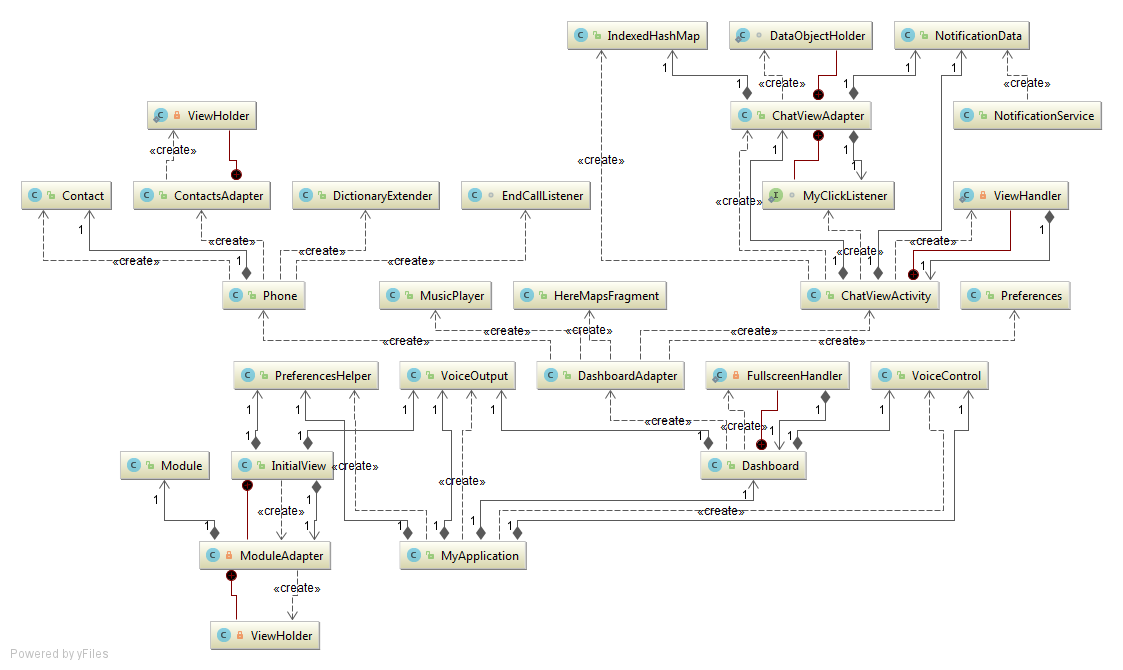
\includegraphics[scale=0.5]{images/diagram.png}
	\caption{Klassen Diagramm}
	\label{figClassDiagram}
\end{figure}

Die Klasse MyApplication dient repräsentativ für die Applikation \ac{ANNA}. Es gibt nur eine Instanz dieser Klasse und entspricht somit dem Programmierparadigma Singleton.\\
Durch den Start der Anwendung, wird durch das Android Betriebssystem eine Objekt dieser Klasse initialisiert. Anschließend werden Instanzen aller Klassen erstellt, welche häufig von anderen Objekten verwendet werden. Über den Aufruf der Instanz von MyApplication, ist es somit anderen Objekten möglich auf Funktionalitäten wie Sprachausgabe, Sprachsteuerung und den Applikationskontext zuzugreifen.\\
Die Klasse MyApplication dient somit als zentrale Schnittstelle für den internen Zugriff der bereitgestellten Funktionalitäten.

Die Klasse InitialView dient als Controller der Oberfäche die dem Nutzer bei erstmaliger Inbetriebnahme der Applikation angezeigt wird. Eine nähere Beschreibung dieser Oberfläche erfolgt in Kapitel \ref{initScreen}.\\
In der Klasse InitialView werden die auf dem Smartphone installierten Module gescannt und die für den korrekten Ablauf der Anwendung nötigen Zugriffsrechte erlangt. Eine genauere Erläuterung der Auffindung installierter Apps auf dem Smartphone wird in Kapitel \ref{installedApps} geschildert.

Die bei der Initialisierung ausfindig gemachten Apps werden durch Objekte der Klasse Module repräsentiert. Diese Klasse liefert eine Liste aller Module-Objekte für die weitere Verwenudung innerhalb der Applikation, als auch die wichtigsten Informationen zu den jeweiligen Modulen. Zu diesen Informationen zählen der Name des Moduls, der Packetname aus Gründen der besseren Identifikation, das Icon des jeweiligen Moduls als auch den aus der Wahl des Nutzers resultierenden Status des Moduls.

Nach der Initialisierung der Anwendung wird eine Instanz der Klasse Dashboard als Controller der Dashboard-Ansicht initialisiert. Die erzeugte Instanz stellt eine Art Container für die Anzeige der Modul spezifischen Benutzeroberflächen dar.\\
Unter Verwendung der Klasse DashboardAdapter werden Instanzen der bereits erwähnten spezifischen Benutzeroberflächen und deren Controller initialisiert und in den Dashboard-Container geladen. Damit dies möglich ist, sind die erwähnten Controller als Sohnklassen der durch Android bereit gestellten Klasse Fragment realisiert.

Eine der Modul spezifischen Controller stellt die Klasse HereMapsFragment da.\\
Die Klasse integriert das HereMaps SDK und stellt Funktionalitäten zur Berechnung von Routen sowie der Turn-by-Turn-Navigation zur Verfügung.

Die Klasse ChatViewActivity dient der Realisierung aller Messenger-Module.\\
Diese Klasse implementiert Methoden zur Benachrichtigung des Nutzers im Falle einer neuen eingehenden Nachricht durch eins der Messenger-Module und um auf diese zu Antworten. Hierfür nutzt die Klasse ChatViewActivity die Klassen ChatViewAdapter, und NotificationData.

Die Klasse ChatViewAdapter ist eine Hilfsklasse zur Visualisierung der eingegangenen Nachrichten. Hierfür führt die Klasse eine interne Liste mit allen Nachrichten und deren angezeigter Position in der Benutzeroberfläche. Zu diesem Zweck verwendet der ChatViewAdapter eine Instanz des selbst erstellten Datentyps IndexedHashMap.

Eingegangenen Benachrichtigungen werden durch die Klasse NotificationData repräsentiert.\\
Objekte dieser Klasse enthalten den Text und den Titel der eingegangenen Benachrichtigungen, den Namen der App, welche die Benachrichtigung erzeugt hat sowie eine Referenz auf das WearableExtender-Objekt, welches die Möglichkeit bietet direkt auf eine Benachrichtigung zu antworten.

Das instantiieren neuer NotificationData-Objekte erfolgt durch die NotificationService-Klasse.
Diese Klasse wird als Listener-Service im Android System registriert, woraufhin das Betriebssystem Android im Falle einer neu eingegangenen Benachrichtigung die Methode onNotificationPosted aufruft. Daraufhin werden die für die NotificationData benötigten Attribute aus der eingegangenen Benachrichtigung extrahiert und der Nutzer über die ChatViewActivity Klasse über den Erhalt einer neuen Benachrichtigung in Kenntnis gesetzt.

Eine weiter Modul-Klasse stellt die Klasse Phone dar.\\
Mittels dieser Klasse wird es dem Nutzer ermöglicht Telefonanrufe zu tätigen sowie SMS-Nachrichten zu versenden.\\
Um diese Funktionalitäten umzusetzen bedient sich die Klasse einiger weiterer Klassen und deren Funktionalitäten.

Eine dieser Klassen ist die Klasse Contact.\\
Sie repräsentiert die im Telefonbuch des Nutzerrs vorhandenen Telefonkontakte. Zu diesem Zweck wird bei der Initiierung der Klasse zunächst mit Hilfe von Threads in einem mehr schrittigen Verfahren das Telefonbuch des Nutzers ausgelesen und anschließend die erstellte Kontaktliste mit Hilfe der Klasse ContactsAdapter dem Nutzer in der Dashboard-Ansicht angezeigt.

Um sicherzustellen, dass die Sprachsteuerung auch für die Kontaktbasierten operationen wie anrufen und SMS senden funktioniert, wird die Klasse DictionaryExtender benötigt.\\
Ihre Aufgabe ist es sicherzustellen, dass die Namen der Kontakte der verwendeten Speech-API bekannt sind. Zu diesem Zweck ergänzt die Klasse die Einträge des Wörterbuchs der verwendeten Speech-API um die gefundenen Namen der Kontakte.

Die Sicherung der Einstellungen erfolgt durch die Klassen Preferences und PreferencesHelper.\\
Die Klasse PrefererncesHelper dient Ausführung der Speicher- und Ladeoperationen der Daten aus dem Sekundärspeicher, während die Klasse Preferences vor allem als Controller für die Benutzeroberfläche des Reiters Einstellungen dient.

\section{Benutzeroberfläche}
Im Rahmen dieser Sektion wird die Benutzeroberfläche für das Projekt \ac{ANNA} beschrieben. Dabei wurde das \ac{UI} maßgeblich von den Zielen von \ac{ANNA} beeinflusst. Deshalb werden diese Ziele zu jederzeit deutlich und weisen stets auf die Absicht der Applikation hin. 
%Leicht lesbar auf Entfernung

\subsection{Material Design}
%https://material.io/guidelines/
Mit der Entwicklung der Android Plattform und der damit verbundenen Vielzahl von Applikationen, welche sowohl von Google als auch von Drittanbietern stammen, wurde eine bildliche Sprache zur Benutzeroberflächen-Vereinheitlichung entwickelt.

Diese visuelle Sprache, welche für die Benutzer der Android Plattform entwickelt wurde, führt die klassischen Prinzipien des guten Designs mit der Innovation und der Möglichkeit von Technik und Wissenschaft zusammen.
Das Synonym dieser Sprache ist Material Design.

Für die Benutzung von Material Design stehen drei Prinzipien im Vordergrund: \textbf{Material ist eine Metapher}, \textbf{Fett, Grafisch, Absichtlich} und \textbf{Bewegung gibt Bedeutung}. Die Metapher ist die vereinigende Theorie eines rationalisierten Raumes und einem Bewegungssystems. Die Grundlagen von Licht, Oberfläche und Bewegung sind der Schlüssel zur Vermittlung, wie sich Objekte im Raum und in Beziehung zueinander bewegen, interagieren und existieren. Im zweiten Prinzip schaffen die verschiedenen Elemente wie Gitter, Raum, Skalierung, etc. vielmehr als nur eine visuelle Begleitung für das Auge zu sein. Diese erzeugen Hierarchie, Bedeutung und Fokus. Durch eine Betonung auf Benutzeraktionen wird die Kernfunktionalität sofort sichtbar und liefert Wegpunkte für den Benutzer. Das letzte Prinzip ist die Respektierung und Stärkung der Bewegung des Anwenders als Hauptantrieb. Primäre Benutzeraktionen sind Wendepunkte, die Bewegung initiieren und das gesamte Design verwandeln.


\ac{ANNA} wird nach den Prinzipien der Material Design Richtlinien entworfen und entwickelt werden, um eine ansprechende und für den Nutzer leicht zu verstehende Benutzeroberfläche zu schaffen, da dieser insbesondere im Straßenverkehr seinen Fokus auf die Straße richten soll. 

\subsection{Initial Screen}
\label{initScreen}
Einer der Kernideen von \ac{ANNA}, wodurch sich das Projekt von bestehenden Applikationen abhebt, ist die Modularität. So können dem Benutzer nur relevante Daten angezeigt und eine Performancesteigerung in Hinblick auf die Spracherkennung angeboten werden, da sich der Kontext proportional zur Anzahl externer Applikationen vergrößert.

Um diese beschriebene Modularität zu erreichen, muss der Nutzer dazu in der Lage sein, seine bestehenden Applikationen, welche im Projekt unterstützt werden, auszuwählen. Dafür wird dem Nutzer wie in Grafik \ref{figInitView} zu sehen, eine Liste mit den verschiedenen Applikationen angezeigt. Diese Liste wird zudem minimal gehalten, da nur bereits installierte Applikationen darin auftauchen. Die genaue technische Umsetzung ist in Sektion \ref{installedApps} zu finden. 

Nach dem auswählen der verschiedenen Applikationen und den zuvor genehmigten Berechtigungen, wird man durch das betätigen eines Buttons zur Home View weitergeleitet, welche je nach Auswahl die Chat View und die Navigation View beherbergt. Nach erstmaliger Modul Konfiguration kann die Selektion im Einstellungsreiter wieder geändert werden.

\begin{figure}[h]
	\centering
  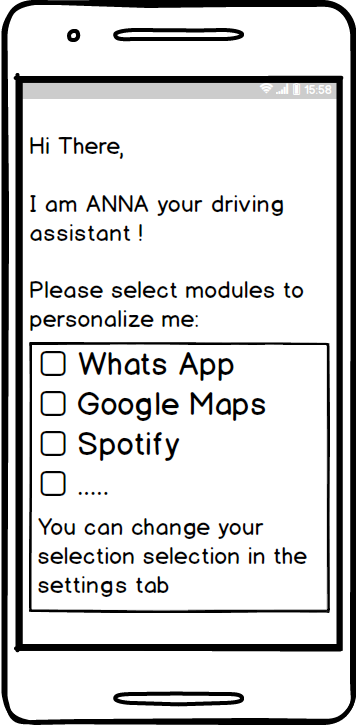
\includegraphics[scale=0.5]{images/initScreen.png}
	\caption{Initiale View}
	\label{figInitView}
\end{figure}

\subsection{Chatview}
Die Chat View verwaltet sämtliche eingehende und ausgehende Nachrichten, um den Fokus auf die Straße zu lenken. Hierbei werden eine Vielzahl von modernen Messengern unterstützt wie beispielsweise Whats App, Allo, Hangouts, Signal, Wire, Messenger und viele weitere. 

Für eine klare Strukturierung der verschiedenen Nachrichtenverläufe wurden sogenannte Cards benutzt, welche ein anpassbares Oberflächen-Element von Android darstellen. Die Cards haben hierbei eine spezielle Struktur, wodurch sich das Element in 5 Sektionen unterteilt. Diese Sektionen sind Profilfoto, Name und Nachricht des Senders, sowie das Logo des benutzen Messengers und die eingehende Uhrzeit der Nachricht. Die beschriebene Strukturierung ist in Grafik \ref{figChatView} zu sehen. Je nach Auflösung des Bildschirms des benutzten Gerätes werden verschieden viele eingegangene Nachrichten angezeigt.

Durch die genaue Strukturierung wird stets ein guter Überblick über die View gewährleistet. Zusätzlich wird dem Nutzer die Möglichkeit gegeben auf ältere Nachrichten zu antworten, da er die Namen der Sender sehen kann. 

\begin{figure}[h]
	\centering
  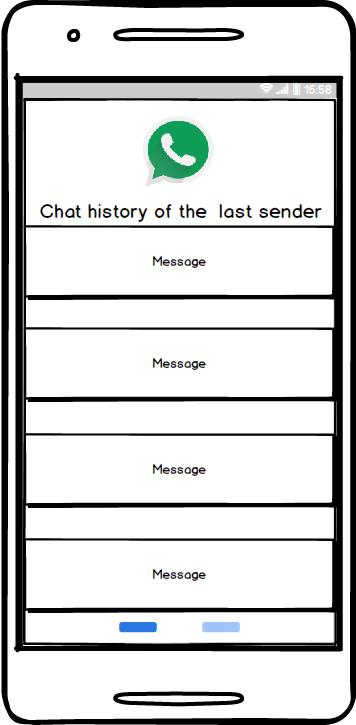
\includegraphics[scale=0.5]{images/WhatsAPP.png}
	\caption{Chat View}
	\label{figChatView}
\end{figure}

\subsection{Navigation}
Die Navigations View beinhaltet einen Navigations-Service, welcher Here Maps ist. Die Wahl des entsprechenden Services findet im Initialen Screen, \ref{figInitView}, statt. 

Nach anfänglicher Auswahl ist diese View, die standardmäßig mittlere View. Das bedeutet immer wenn die App gestartet wird, wird der Navigationsservice das erste sein, dass der Nutzer sieht. Durch die Integrierung der Applikationen wie Here Maps als Service ist es möglich alle spezifischen Funktionalitäten zu nutzen. Dies ist auf der Grafik \ref{figNavigation} zu erkennen, die einen Beispielbetrieb im Navigationsmodus des Services zeigt.

Die Spracheingabe wird jedoch über die Sprach API \ac{CMU} gehandhabt, da gewünschte Funktionalitäten nicht vorhanden sind oder Datenvolumen bereits bei der Sprachberechnung verbraucht wird. 

\begin{figure}[h]
	\centering
  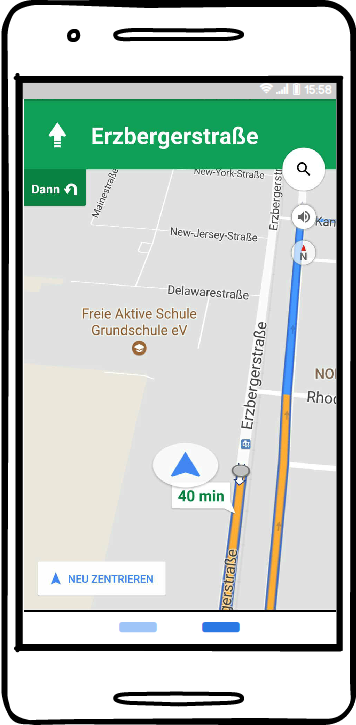
\includegraphics[scale=0.5]{images/Navigation.png}
	\caption{Navigations View}
	\label{figNavigation}
\end{figure}

\subsection{Menüführung}
Die Menüführung befasst sich mit der Navigation zwischen den verschiedenen Ansichten der Applikation. Dabei wird eine berührungslose Navigation, durch Spracheingabe und eine Navigation über den Touchscreen unterstützt.

Die berührungslose Interaktion zum Wechseln der Views, wird durch Befehle wie ,,Zeige mir die letzte View'' oder auch ,,Wechsle zur Navigationsansicht'' gesteuert. Allerdings muss der Nutzer wie bei allen anderen Befehlen das System mit dem Hotword ,,ANNA'' zunächst aus dem Schlafmodus wecken.

Im Unteren Bereich des Bildschirms befindet sich die Anzeige, welche View gerade ausgewählt ist, siehe Grafik \ref{figNavigation} und \ref{figChatView}. Dies ermöglicht eine einfache Erweiterung für neue Applikationen. Zusätzlich schafft es einen schnellen Überblick über die Anzahl der ausgewählten Module.  

Die Steuerung über den Touchscreen durch diese Anzeige sehr intuitiv. Das bedeutet, der Benutzer muss lediglich in die Richtung wischen, in der sich die gewünschte View befindet.

Befindet sich der Nutzer bereits in der am weitesten links befindlichen Ansicht und wischt dann erneut nach links öffnet sich das Einstellungsmenü. Diese Funktionalität ist in Grafik \ref{figSettings} zu sehen. In dieses Menü kann der User zusätzlich über eine Spracheingabe gelangen. Innerhalb des Menüs können Module konfiguriert und Accounts für beispielsweise Spotify oder andere Applikationen, welche Anmeldeinformationen benötigen, verwaltet werden.

\begin{figure}[h]
	\centering
  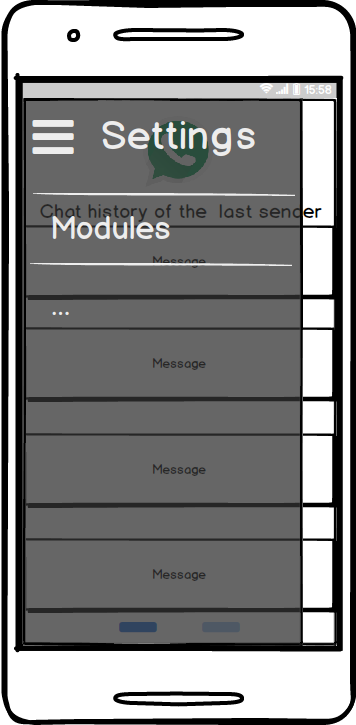
\includegraphics[scale=0.5]{images/Settings.png}
	\caption{Einstellungs View}
	\label{figSettings}
\end{figure}

\subsection{Voice Recognition}
Um das Ziel der Applikation, den Fokus wieder auf die Straße zu lenken, zu erreichen, ist die berührungslose Interaktion unabdinglich. Deshalb nimmt die Spracherkennung auch in der Oberfläche eine wichtige Rolle an. Daraus leitet sich ab, dass der Nutzer Visualisierungen für die Aufnahmefähigkeit des Gerätes und die bereits erkannte Eingabe benötigt.

Diese Visualisierung ist in Grafik \ref{figRecognition} zusehen. Um zu der beschriebenen Ansicht zu gelangen, muss der Benutzer die Spracherkennung durch das Hotword ,,ANNA'' starten. Zusätzlich zur visuellen Bereitschaftsanzeige, siehe Grafik \ref{figRecognition}, bekommt der Nutzer ein auditives Signal um dem Nutzer zu zeigen, dass \ac{ANNA} nun auf seine Spracheingaben reagiert. Dieses Signal kann je nach Einstellungen des Benutzers entweder ein einfacher Ton sein oder eine Sprachausgabe von \ac{ANNA} wie ,,Was kann ich für dich tun'' sein.
Zur Überprüfung der Eingabe kann der Nutzer sich das Gesagte vom System vorlesen lassen. Allerdings kann auf die Überprüfung der Eingabe verzichtet werden.

Durch das Ansprechen visueller und aditiver Wahrnehmung, durch Overlay und Signalton, erkennt der Nutzer jederzeit im Straßenverkehr, ob das System auf das Hotword reagiert hat und sich im Aufnahmemodus befindet, ohne dabei übermäßig abgelenkt zu werden.  
\begin{figure}[h]
	\centering
  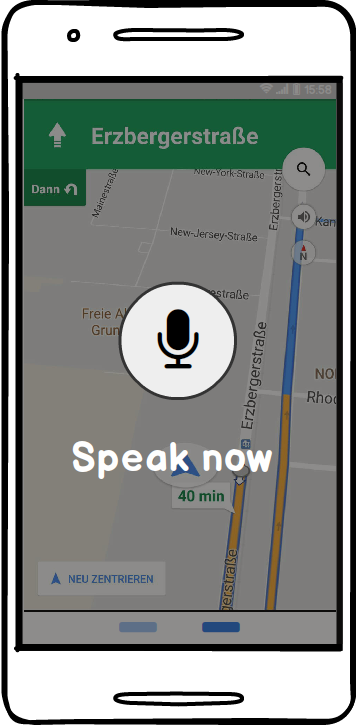
\includegraphics[scale=0.5]{images/voiceRecognition.png}
	\caption{Recognition Overlay}
	\label{figRecognition}
\end{figure}


\section{Modularität}
Bei der Umsetzung des Projekts \ac{ANNA} steht vor allem die Individualität der Nutzer im Vordergrund. Viele Dienste binden den Nutzer an die Verwendung der bereits verknüpfter Applikationen, ohne die Chance zu haben diese aus dem \ac{UI} zu entfernen oder andere vom User bereits benutzte externe Applikationen hinzuzufügen.\\
\ac{ANNA} spiegelt jedoch die Individualisierung der Nutzer wieder. Daher wird der Nutzer bei der erstmaligen Verwendung der Applikation dazu aufgefordert aus einer Liste von Applikationen diejenigen auszuwählen, die er selbst häufig benutzt und deren Unterstützung er sich von seinem persönlichen Fahrassistenten wünscht.\\
Die nach der Auswahl der Applikationen folgenden Benutzeroberflächen werden anschließend auf Basis der vom Nutzer getroffenen Modulwahl generisch zusammengestellt. Dabei ist es wichtig, dass die einzelnen Module unabhängig voneinander agieren, da eine Bereitstellung einzelner Module sonst nicht möglich wäre.

\subsection{Identifizierung externer Applikationen}
\label{installedApps}
Für das Auffinden installierter Applikationen, welche dem Nutzer über den Initial Screen zur Auswahl präsentiert werden, werden zwei verschiedene Methoden genutzt.

Innerhalb der Applikation \ac{ANNA} wird eine Liste mit den Namen der unterstützten Messengers geführt. Bei der Initialisierung der Applikation, werden zunächst alle installierten Apps, mithilfe des von Android bereitgestellten Packagemanager, abgerufen. Zusätzlich ist es mit dem Packagemanager möglich, die Namen der installierten Apps und deren Logos abzurufen. Nachdem die Informationen über die auf dem Geräte installierten Anwendungen zur Verfügung stehen wird überprüft, ob sie in der Liste enthalten sind. Wenn dies der Fall ist, wird ein entsprechendes Objekt instantiiert, welches die dazugehörige Applikation repräsentieren soll. Zu diesem Zweck werden innerhalb des jeweiligen Objektes Metainformationen zur korrespondierenden Anwendung bereitgestellt.

Bei Applikationen aus anderen Kategorien wie beispielsweise der Telefon- oder SMS-App wird ein anderer Ansatz genutzt, um dazugehörigen Anwendungen zu identifizieren.\\
Wie auch bei anderen Betriebssystemen wie beispielsweise Microsoft Windows, gibt es Applikationen die für bestimmte Zwecke oder Formate als Standard zur weiteren Verarbeitung verwendet werden. Dies ist auch bei Android der Fall. Über die Angabe einer bestimmten Kategorie wie beispielsweise \texttt{CATEGORY\_APP\_MESSAGING}, ist es möglich die jeweilige Standard Applikation für die entsprechende Kategorie abzufragen und die dazugehörigen Informationen über den Packagemanager zu erhalten.

\section{Sprachverarbeitung}
\label{languageProcessing}
Eine der wichtigsten Funktionen von Projekt \ac{ANNA} ist die Sprachverarbeitung. Sie ist die primär fokussierte Schnittstelle zur Interaktion zwischen System und Nutzer.

In den nachfolgenden Sektionen werden die einzelnen Bestandteile der Applikation, welche mit Sprachverarbeitung im Zusammenhang stehen sowie die Theroie die hinter der Sprachverarbeitung steht, näher erläutert.

\subsection{Decoding}
Zur Umwandlung von Sprache zur Text wird im Rahmen von \ac{CMU} eine statistische Modellierung namens Hidden Markov Models in Kombination mit Algorithmen verwendet. Ein Markov Model definiert sich dadurch, dass es aus n Zuständen besteht, welche jedoch nicht direkt beobachtet werden können. Dabei emmitiert jeder dieser Zustände zu jedem Zeitpunkt einen zufällig sichtbaren Zustand. Innerhalb der Spracherkennung bietet sich das Hidden Markov Model als mathematische Formulierung besonders in 2 Teilbereichen an. \footcite[vlg.:][S. 1 f.]{hmmIsolated}

Zum einen für ,,Isolated Words'' und zum andern für ,,Continous Speech''. Wie der Name beschreibt, werden bei ,,Isolated Words'' die Wörter einzeln nacheinander getrennt von einer Pause erkannt. Die genaue Berechnung des Wortes ist in Grafik \ref{figIsoRecognition} zu sehen. Dabei wird das eigehende Sprachsignal qunatisiert und somit in Vektoren zerlegt. Da jedes Hidden Markov Model ein Wort representiert wird mit Hilfe eines Algorithmus die Wahrscheinlichkeit ausgerechnet, dass die eingegange Sprachsequenz von einem dieser Model stammt. Das Model, bei dem die höchste Wahrscheinlichkeit besteht, dass die Sequenz von diesem stammt wird ausgewählt und ausgegeben.
\footcite[vlg.:][S. 12 f.]{hmmIsolated}

,,Continous Speech'' Spracherkennung ist jedoch deutlich schwerer, da der Computer im Gegensatz zur ,,isolated recognition'' nicht durch eine Pause signalisiert bekommt, dass das Wort zu Ende ist. Dies bedeutet, dass der Computer selbst entscheiden muss, wann das Wort geendet hat und wann ein neues anfängt. Allerdings ist gerade diese Entscheidungsfähigkeit des Computers unabdinglich im Hinblick auf die Spracherkennung im Projekt, da die Sprachkommandos aus zusammengesetzten Wörtern bestehen.
Im Gegensatz zur Einzelworterkennung repräsentiert wird nicht jedes Wort von einem einzelnen Hidden Markov Model zugeordnet, sondern es wird ein großes Model gebaut, durch das hinzufügen von Übergangszuständen. Spracherkennung auf Basis dieses neu erzeugten Models, funktioniert nun durch das Suchen nach der Sequenz an Zuständen, welche am wahrscheinlichsten mit der Sequenz des gegebenen Beobachtungsvektor übereinstimmt. Diese Wahrscheinlichekiten werden über einene Algorithmus bestimmt. 
\footcite[vlg.:][S. 29 f.]{hmmContinous}

\begin{figure}[h]
	\centering
  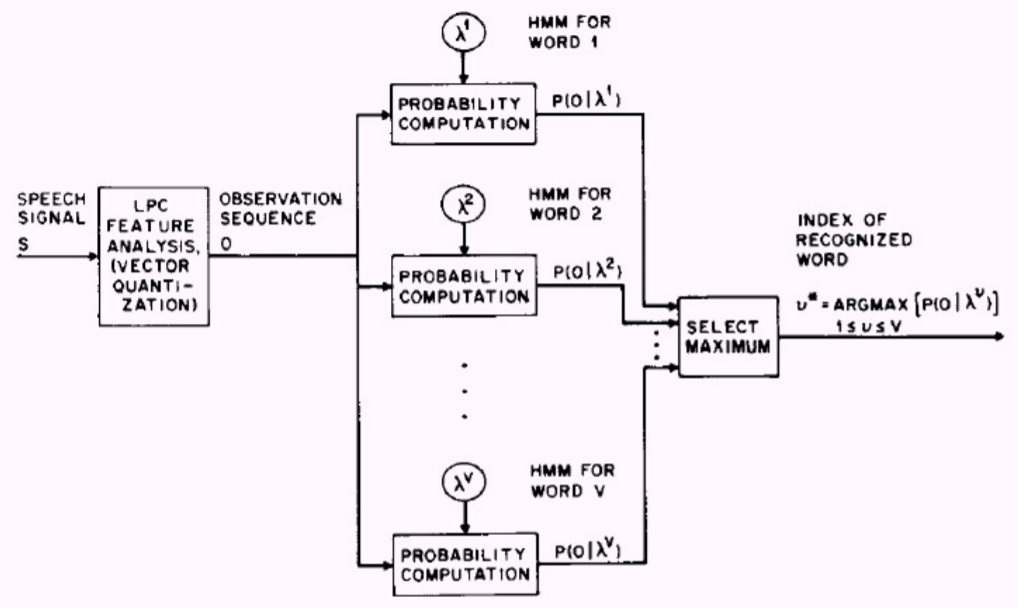
\includegraphics[scale=0.5]{images/iso_word_recog.png}
	\caption{Isolated Word Recognizer}
	\label{figIsoRecognition}
\end{figure}


\subsection{Störgeräuschreduktion}
In einem Sprachsignal sind immer Hintergrundgeräusche enthalten. Diese Hintergrundgeräusche maskieren das eingehende Signal derart, dass Qualitätsverluste die Folge sind. Wenn das Sprachsignal ohne eine Störgeräuschreduktion prozessiert werden würde, wäre die Performance des Systems erheblich schlechter, da dieses falsch Interpretationen aufgrund von Störgeräuschen zusätzlich berechnen würde.
Um diesen Performanceverlust entgegenzuwirken und um eine klareres Bild des Signals zu bekommen, gibt es spezielle Lärmunterdrückungs-Algorithmen. 
\footcite[vlg.:][S. 1 ]{specSub}

Einer dieser Algorithmen ist der, der spektralen Subtraktion. Die spektrale Subtraktion ist den Einzel-Kanal-Sprachverbesserungen zugehörig. Im Gegensatz zur Mehrfach-Kanal-Sprachverbesserung kann mit wenig Aufwand eine akzeptable Trennung von Sprache und Lärm innerhalb eines Signals erreicht werden. Die spektrale Subtraktion findet auch in \ac{CMU}, zur Reduzierung von Hintergrundgeräuschen, Verwendung. 
\footcite[vlg.:][S. 1 ]{specSub}

Um die Störgeräusche herauszufiltern stützt sich die spektrale Subtraktion auf die Formel \ref{noiseSum}. Hierbei setzt sich das unklare, geräuschvolle Signal u(s) aus dem eingehenden Sprachbefehl c(s) und den Hintergrundgeräuschen n(s) zusammen. Um den klaren Sprachbefehl zu bestimmen, wird n(s) geschätzt und vom Signal abgezogen. 
\footcite[vlg.:][S. 2 f.]{specSub}

%\begin{equation}
%    \label{noiseSum}
%    u(s) = c(s) + n(s) 
%\end{equation}

Der Ablauf des Algorithmus ist in Grafik \ref{figspecSub} zu sehen. 
In diesem Fall wird ein unklares, geräuschvolles Signal in meherere kleine Frames zerteilt. Danach wird mit Hilfe der Schnellen Fouriertransformation das Signal in den Frequenzraum transformiert, da sich dort mathematische Operationen leichter anwenden lassen. Die Diskrete Kosinus Transformation wird wiederum dazu genutzt, um die Urpsrungstöne zu finden, welche durch Überlagerungen von Tönen entstanden. Durch die Berechnung der Ursprungstöne und die Analyse der einzelnen Frames kann eine Abschätzung des Hintergrundgeräusches vorgenommen werden. Die Analyse der einzelnen Frames ist unabdinglich, da Frames existieren bei denen zum Zeitpunkt t kein Signal vom Nutzer eingeht und somit das Signal als Hintergrundgeräusch gedeutet werden kann.
Ausgehend von den Berechnungen wird nun ein gewisser Prozentsatz des Hintergrundgeräusches ne(w) vom Eingangssignal m(w) abgezogen. Um nun zu c(s) aus Formel \ref{noiseSum} zugelangen, muss das Signal wieder zurück transformiert werden. Nun steht dem Decoding des eigegangenen Signals nichts mehr im Weg.
\footcite[vlg.:][S. 2 f.]{specSub}
\footcite[vlg.:][]{fft}
\footcite[vlg.:][]{dct}

\begin{figure}[h]
	\centering
  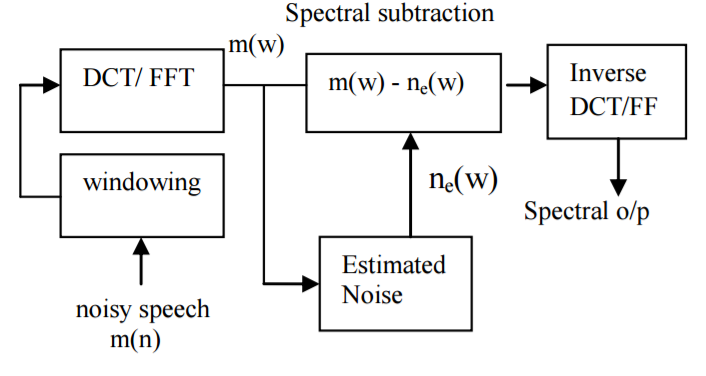
\includegraphics[scale=0.7]{images/spectral_sub.png}
	\caption{Sequenz Diagramm der Spektralen Subtraktion}
	\label{figspecSub}
\end{figure}

\subsection{Spracherkennung}
Die Erkennung der gesprochenen Sprache erfolgt anhand der durch den User eingestellten Systemsprache des Geräts.\\
Bei der Initialisierung der Speech Engine wird zunächst, über eine von Android bereit gestellte Funktion, die eingestellte System Sprache abgefragt, um anhand dieses Ergebnisses die entsprechenden Sprachbibliotheken und definierten Grammatiken zu laden.\\
Für den Nutzer bietet dies den Vorteil sich nicht mit zusätzlichen Einstellungen beschäftigen zu müssen und ein besseres Ergebnis bei der Sprach in Textumwandlung zu erhalten. Diese Vorgehensweise hat jedoch auch einen negativen Aspekt. Da die Systemsprache eindeutig ist und es beim aktuellen Stand nicht möglich multilingual mit dem System zu interagieren. Eine Eingabe in einer Sprache, welche nicht der Systemsprache entspricht, erzielt somit weniger bis gar keine genauen Ergebnisse bei der Umwandlung in Text.

Um den benötigten Speicher sowie die Komplexität im Rahmen dieser Studienarbeit gering zu halten, bietet die Spracherkennung zunächst nur die Erkennung für die Sprachen Deutsch und Englisch an.\\
Je nach voranschreiten der Entwicklung und der verbleibenden Zeit werden weitere Sprachen unterstützt.

\subsection{Hotword Detection}
\label{scthotword}
Um das Ziel der Reduzierung von Verkehrsunfällen durch Smartphone Interaktionen zu minimieren, ist es wichtig jegliche Berührung des Smartphones und der damit verbundenen Ablenkung vom Straßenverkehr zu reduzieren.\\
Die in diesem Kapitel beschriebenen Spracherkennungsfunktionen sind ein wichtiger Schritt hin zur Erfüllung dieses Ziels.\\1
Viele Speech-to-Text Dienste funktionieren an dieser Stelle auf die Weise, dass der Nutzer zunächst einen Knopf betätigen muss um die Sprachaufnahme und die damit verbundenen Umwandlung in Text zu starten. Bei einigen Tools ist es sogar notwendig für die Dauer der Sprachaufnahme den entsprechenden Knopf gedrückt zu halten.\\
Ein solches Verfahren ist für Projekt \ac{ANNA} eher ungeeignet, da der Nutzer des öfteren den Blick von der Straßen weg hin zu seinem Smartphone richten müsste um den entsprechenden Knopf ausfindig zu machen und diesen zu drücken.\\
Um dieses Problem zu umgehen, kommt an dieser Stelle eine Hotword Detection zum Einsatz.

Als Hotword Detection bezeichnet man die Suche nach einem bestimmten Wort oder einem kurzen Satz in einem kontinuierlich aufgenommenen Audiostream.\\
Hierzu wird sobald die Applikation gestartet wurde und die erstmalige Initialisierung abgeschlossen ist, die Speech-to-Text Engine initialisiert und kontinuierlich alle eingehenden Audiosignale auf das Auftreten des definierten Hotword geprüft.\\
Wird das Hotword nicht erkannt, werden die Aufnahmen ohne weiter Verarbeitung verworfen. Sobald jedoch das Hotword erkannt wurde, startet die interne sprachbasierte Menüführung zur Identifikation der vom Nutzer gewünschten Aktion. Weitere eventuell benötigte Informationen werden über einen Dialogmodus, im Sinne von Frage durch das System und Antwort des Nutzers, in Erfahrung gebracht.

\subsection{Kontext basierte Grammatiken}
Betrachtet man die reale Welt, bemerkt man schnell, dass die Reihenfolge sowie die Anzahl der sinnvoll zu verwendeten Wörter durch die jeweilige Situation eingeschränkt sind. Diese Erkenntnis lässt sich auch bei der Spracherkennung anwenden.\\
Betrachtet man zum Beispiel folgendes Szenario: Ein Nutzer möchte ein Telefonat führen und diktiert die Telefonnummer die er anrufen möchte. Da Telefonnummern nur aus Zahlen bestehen und gegebenenfalls aus einem Plus für die Landesvorwahlen, lässt sich der Umfang der für die Speech-to-Text Engine zu prüfenden Wörter entsprechend auf Zahlen reduzieren, wodurch die Genauigkeit der erfolgreichen Speech-to-Text Umwandlung erhöht wird.

Die Einschränkung der zu überprüfenden Wörter erfolgt hierbei durch die Definition verschiedener Grammatiken, welcher in einer Backus-Naur ähnlichen Form definiert werden.\\
Die so definieren Grammatiken können dann je nach Kontext in dem sich der User durch seine vorherige Spracheingabe befindet geladen werden, um die jeweilige Genauigkeit bei der Spracherkennung zu erhöhen.\\
Zur Veranschaulichung der Struktur einer solchen Grammatik, zeigt Listing \ref{lstGrammar} eine simple Grammatik zur Erkennung einer einfachen Telefonnummer. Die für CMU Sphinx verwendeten Grammatiken werden dabei alle in \ac{JSGF}-Dateien definiert.

\begin{lstlisting}[caption={Einfache Grammatik zur Erkennung von Telefonnummern},captionpos=b,label=lstGrammar]
#JSGF V1.0 ISO8859-1 de;

grammar call;

public <number> = <digit>*;
<digit> = eins | zwei | drei | vier | fünf | sechs | sieben | acht | neun | null;
\end{lstlisting}

\section{Benachrichtigungsverarbeitung}
Zur Reduzierung der Ablenkung des Nutzers während der Fahrt durch neue Benachrichtigungen auf dem Smartphone, werden diese abgefangen und dem Nutzer auf Wunsch vorgelesen und die Möglichkeit geboten direkt auf diese zu antworten.

Um neue Benachrichtigungen abzufangen wird ein Notification Listener instanziiert. Damit dieser Zugriff auf eingehende Benachrichtigungen erhält, muss der Nutzer zunächst die entsprechende Einstellung an seinem Smartphone durchführen. Zur Erleichterung dieses Schrittes, wird der Nutzer während der erstmaligen Inbetriebnahme der Applikation durch die nötigen Konfigurationsschritte geführt.

Nach der erfolgreichen Konfiguration und der Gewährung aller nötigen Berechtigungen, ist der Notification Listener bereit neue Benachrichtigungen abzufangen und die Applikation ist somit in der Lage, den in Graphik \ref{figNotification} dargestellte Programmablauf auszuführen. Geht eine neue Benachrichtigung am Smartphone ein, wird per Broadcast an alle registrierten Notification Listener gesendet. Diese bieten, da sie von der abstrakten Klasse \texttt{NotificationListenerService} erben, verschiedene Methoden welche bei einer Veränderung des Status einer Benachrichtigung aufgerufen werden. Mögliche Beispiele wären hier die Methoden \texttt{onNotificationPosted}, welche aufgerufen wird wenn eine neue Benachrichtigung im System eingeht oder die Methode \texttt{onNotificationRemoved}, die beim Entfernen einer Benachrichtigung aufgerufen wird.

Stellt der Notification Listener fest, dass eine neue Benachrichtigung vom System eingegangen ist, prüft die Applikation zunächst ob es sich beim Erzeuger der Benachrichtigung um eine Applikation handelt, welche vom Nutzer als Modul aktiviert wurde. Trifft dieser Fall ein, wird die Benachrichtigung vom System abgerufen und zunächst zur besseren Verarbeitung in ein applikationsinternes Datenformat transformiert. Anschließend wird dem Nutzer mittels Text-to-Speech Engine der Titel der Benachrichtigung vorgelesen. Bei dem Titel einer solchen Benachrichtigung handelt es sich um Informationen, die benötigt werden um den restlichen Inhalt einer Benachrichtigung zuordnen zu können. Bei einer eingehenden WhatsApp Nachricht, würde dieser Titel wie folgt lauten: Eine neue Nachricht von Max Mustermann.\\
Der Nutzer wird anschließend wiederum per Text-to-Speech Mechanismus gefragt ob er den Inhalt der Nachricht vorgelesen bekommen möchte. Die Antwort des Nutzers wird dann wiederum per Speech-to-Text Engine umgewandelt. Sollte das Ergebnis dieser Antwort positiv sein, wird die Nachricht vorgelesen und der Nutzer weiterhin gefragt ob er auf diese Nachricht antworten möchte.\\
Für die Text-to-Speech Umwandlung wird einfachheitshalber die vom Nutzer primär eingestellte Text-to-Speech Engine verwendet. Für die Auswertung der Antworten des Nutzers wird das Framework CMU Sphinx verwendet, welches in Sektion \ref{sctcmu} näher beschrieben wird.

\begin{figure}[h]
	\centering
  \includegraphics[scale=0.5]{images/notification.png}
	\caption{Ablaufsdiagramm für den Eingang einer neuen Benachrichtigung}
	\label{figNotification}
\end{figure}

Die Vorlesefunktion neuer Benachrichtigung funktioniert mit jeder gängigen Applikation, da es sich bei dem Abfangen neuer Benachrichtigungen um eine Android spezifische Standardfunktion handelt.\\
Gerade bei Messenger Diensten, variiert jedoch die Offenheit der Messenger gegenüber der Nutzung durch dritte. Einige Dienste bieten hier eigene \ac{API}s an um mit den Messenger Dienst zu interagieren, andere wie beispielsweise der populäre Dienst WhatsApp jedoch, bieten keinerlei offizielle Schnittstelle für die Nutzung durch dritte.\\
Um den Entwicklungsaufwand an dieser Stelle in einem vertretbaren Maße zu halten und gleichzeitig möglichst viele Messenger zu unterstützen ohne, dass selbst der exotischste Messenger bekannt sein muss, wird an dieser Stelle ein Workaround angewendet.\\
Mit der Einführung von Android Wear und den damit erschienen \gls{Wearables}, entwickelte Google eine neue Datenstruktur, welche speziell für das anzeigen und Antworten über Wearables konzipiert ist. Diese Datenstruktur enthält eine Referenz, welche es ermöglicht gezielt auf eine neue Nachricht von einem bestimmten Kontakt aus dem jeweiligen Messenger zu antworten. Diese neue Datenstruktur, welche als \texttt{WearableExtender} bezeichnet wird, wird im Benachrichtigungsobjekt referenziert.\\
Geht nun eine neue Benachrichtigung ein, wird das \texttt{WearableExtender} Objekt, welches normalerweise an ein Wearable Gerät gesendet werden würde aus dem Benachrichtigungsobjekt extrahiert und für die direkte Interaktion mit den jeweiligen Messenger und speziell mit dem jeweiligen Kontakt verwendet.\\
Deshalb ist es nicht mehr erforderlich die Unterstützung für jeden Messenger einzeln zu implementieren und sich mit deren Funktionsweise auseinanderzusetzen.
